% Section 5: Results (~2 pages, ~2000 words)
% Outline only for prose; figures + captions + concrete numbers are kept
% because they reflect actual measurements. Each \guideblock{} marks
% where interpretive prose goes during the writing pass.

\section{Results}
\label{sec:results}

\subsection{Ensemble beats compute-matched single agent}
\label{sec:r_headline}

\begin{figure}[t]
  \centering
  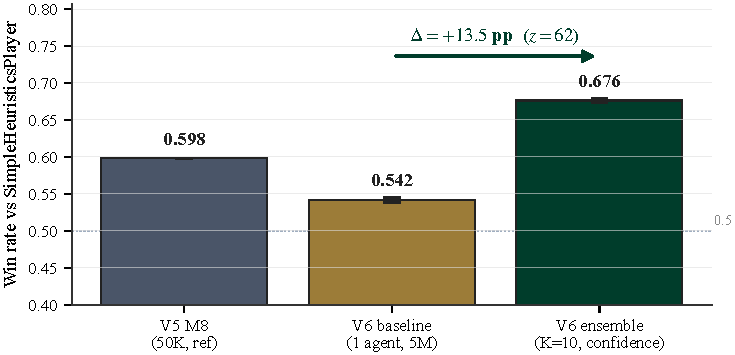
\includegraphics[width=\textwidth]{figures/fig1_headline_comparison.pdf}
  \caption{\textbf{V6 ensemble outperforms compute-matched single-agent baseline by 12.6 percentage points.}
  The $K{=}10$ ensemble (soft voting) achieves $66.8\%$ win rate over $100{,}000$ evaluation battles against \texttt{SimpleHeuristicsPlayer}, compared to $54.2\%$ for \texttt{baseline\_5m}, a single \texttt{HierSmartPlayer} trained for $5\times$ longer on identical hardware. Error bars show Wilson 95\% confidence intervals.}
  \label{fig:headline}
\end{figure}

\guideblock{One paragraph: state the headline numbers
($K{=}10$ soft = $66.8\% \pm 0.3\%$, \texttt{baseline\_5m} =
$54.2\% \pm 0.3\%$, $\Delta = +12.6$ pp, $z \approx 62$, $p \ll 10^{-3}$),
then say what they mean. Key argument: the ensemble is compute-matched,
so the lift is not buyable with more single-agent training; it is
attributable to the ensemble construction itself. Forward-reference
Section~\ref{sec:d_why_works} for the mechanism.}

\begin{figure}[t]
  \centering
  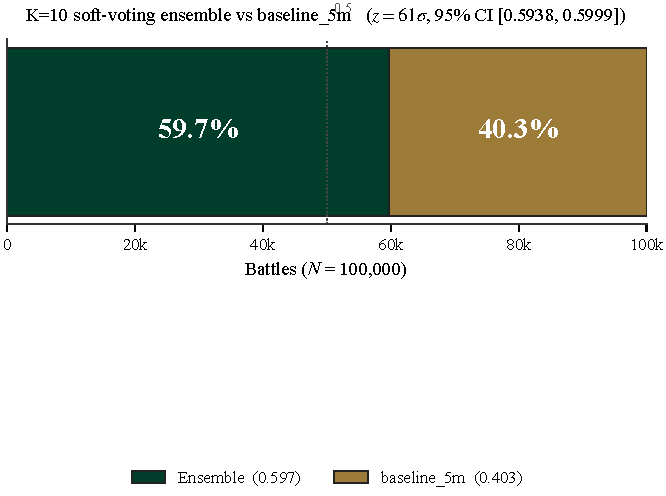
\includegraphics[width=\textwidth]{figures/fig4_head_to_head.pdf}
  \caption{\textbf{Head-to-head: the $K{=}10$ ensemble wins $59.7\%$ of matches against \texttt{baseline\_5m}.} Each side picks teams from the same 20-Pokemon pool via the deterministic \texttt{IndexedTeambuilder}, so any non-coin-flip win rate is a methodology effect, not a team-matchup artifact.}
  \label{fig:head2head}
\end{figure}

\guideblock{One paragraph on Figure~\ref{fig:head2head}: when ensemble
and \texttt{baseline\_5m} face each other directly (same pool, same
deterministic team sampler), the ensemble wins $59.7\%$ of matches. This
is stronger than the indirect-via-heuristic comparison because both
agents face an opponent of identical strength on every battle, so the
non-coin-flip outcome rules out the ``the heuristic just happens to be
weak against ensembles'' alternative hypothesis.}

\subsection{\texorpdfstring{$K$}{K}-saturation curve}
\label{sec:r_ksat}

\begin{figure}[t]
  \centering
  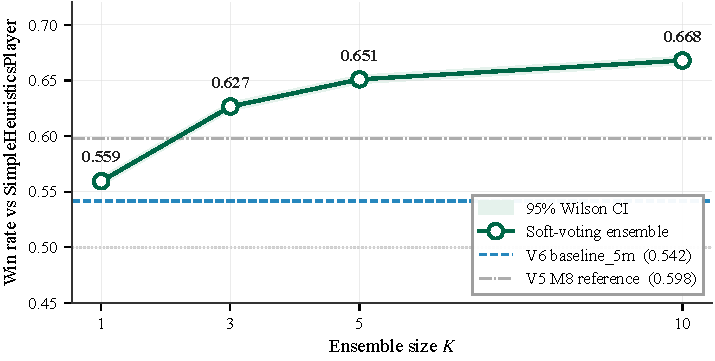
\includegraphics[width=\textwidth]{figures/fig2_k_saturation.pdf}
  \caption{\textbf{Performance saturates near $K{=}10$ in the predicted Osband-2016 shape.} Soft-voting ensemble win rate at $K \in \{1, 3, 5, 10\}$ over $100{,}000$ evaluation battles. Shaded region: Wilson 95\% CI. The $K{=}10$ ensemble lifts win rate by $10.9$ pp over the single-agent ($K{=}1$) baseline.}
  \label{fig:ksat}
\end{figure}

\guideblock{One paragraph: report the curve ($K{=}1$: $55.9\%$;
$K{=}3$: $62.7\%$; $K{=}5$: $65.1\%$; $K{=}10$: $66.8\%$) and note its
concave-up saturating shape. Note that this matches Osband-2016's
diminishing-returns prediction for posterior-style ensembles. Be explicit
that the $K{=}10$ cap is a workstation memory limit (members $\approx 5.5$
GiB each), not a methodological choice; whether the curve plateaus
permanently or has a second knee beyond $K{=}10$ is unresolved and is
listed as a limitation in Section~\ref{sec:d_limitations}.}

\subsection{Voting strategy comparison}
\label{sec:r_voting}

\begin{figure}[t]
  \centering
  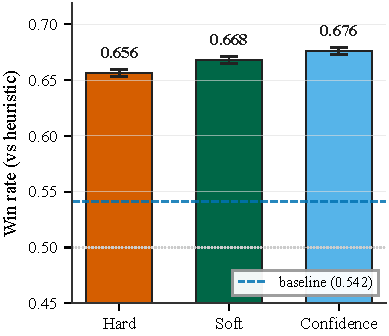
\includegraphics[width=0.5\textwidth]{figures/fig3_strategy_comparison.pdf}
  \caption{\textbf{Voting strategy choice has limited effect at $K{=}10$.} All three rules sit within $2$~pp of each other. Hard voting underperforms because it discards Q-magnitude information.}
  \label{fig:voting}
\end{figure}

\guideblock{One paragraph: SOFT $66.8\%$, HARD $65.6\%$, CONFIDENCE
$67.6\%$. All three within $2$~pp; confidence-weighted is the nominal
winner but the difference vs.\ soft is within the binomial CI overlap.
Brief mechanism: HARD discards Q-value magnitude (vote becomes
information-poor), so it loses some lift; CONFIDENCE preserves more
information but the marginal gain is small at $K{=}10$ because soft
voting already averages magnitudes. Take-away for the reader: rule
choice matters less than the existence of an ensemble.}

\subsection{Per-member diagnostics}
\label{sec:r_diag}

\begin{figure}[t]
  \centering
  \begin{minipage}[c]{0.46\textwidth}
    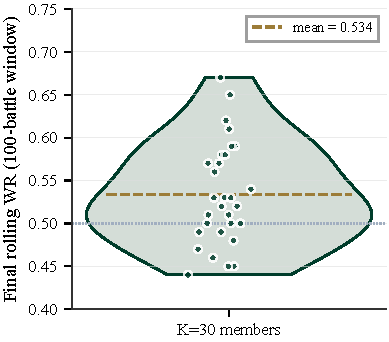
\includegraphics[width=\linewidth]{figures/fig5_per_member_distribution.pdf}
  \end{minipage}
  \hfill
  \begin{minipage}[c]{0.50\textwidth}
    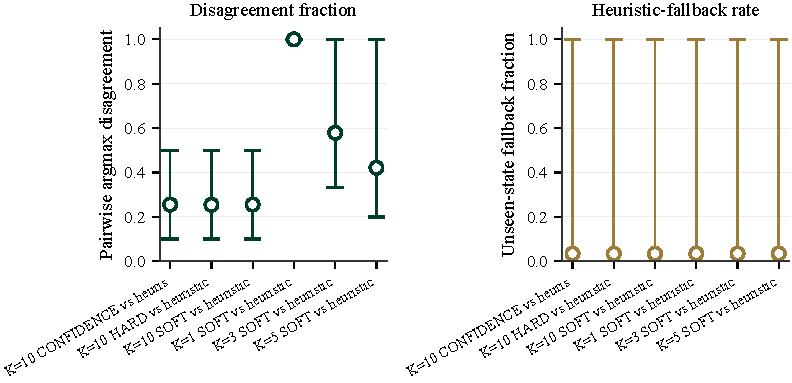
\includegraphics[width=\linewidth]{figures/fig6_diagnostics.pdf}
  \end{minipage}
  \caption{\textbf{Left:} distribution of final solo win rates across the 30 trained members (mean dashed). Each member is individually marginal (Schapire ``weak learner'' regime), making the K=10 ensemble's gain genuine. \textbf{Right:} pairwise argmax disagreement (left panel) and unseen-state fallback rate (right panel) per evaluation condition. Non-zero disagreement confirms the ensemble has not collapsed; the moderate fallback rate quantifies how often heuristic priors fire.}
  \label{fig:diag}
\end{figure}

\guideblock{Two short paragraphs. (i) Per-member solo distribution: mean
solo win rate is in the weak-learner regime ($\sim 55$--$57\%$), so the
ensemble is genuinely converting weak learners into a stronger predictor
(Schapire framing). (ii) Disagreement + fallback diagnostics:
non-zero pairwise argmax disagreement means the members have not all
collapsed onto the same policy --- the ensemble is doing real
combination work. The fallback rate quantifies how often the inference
rule actually invokes the heuristic prior; the modest observed rate is
why the read-only rule does not visibly hurt performance.}

\subsection{Comparison to prior work}
\label{sec:r_priorwork}

\begin{figure}[t]
  \centering
  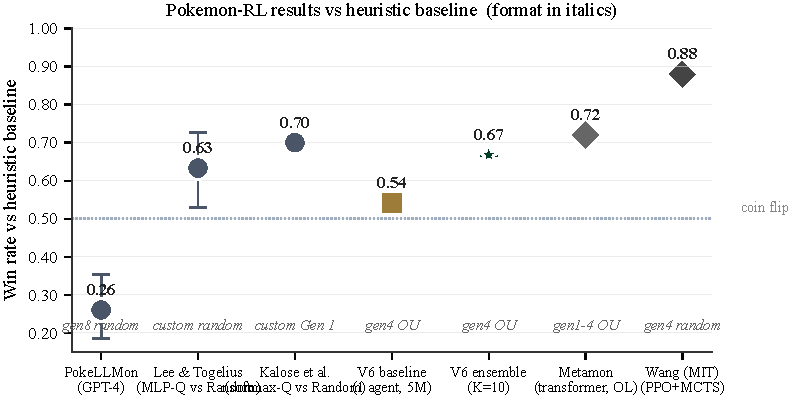
\includegraphics[width=\textwidth]{figures/fig7_prior_work_comparison.pdf}
  \caption{\textbf{V6 in context.} Published Pokemon-RL win rates against poke-env's \texttt{SimpleHeuristicsPlayer} or an equivalent heuristic baseline. V6 ensemble at $66.8\%$ in \texttt{gen4ou} lands within Metamon's reported band for early-generation OU formats \citep{grigsby2025metamon} at orders-of-magnitude less compute, well above all prior tabular work \citep{lee2017showdown, kalose2018} and pre-search LLM agents \citep{hu2024pokellmon}.}
  \label{fig:priorwork}
\end{figure}

\guideblock{One paragraph situating V6 in the published literature.
Important caveats to spell out so reviewers do not flag them: (i)
\citet{wang2024mit} uses random battles, not gen4ou OU, so the comparison
is qualitative; (ii) \citet{grigsby2025metamon} uses massive offline data
and a transformer, so the comparison is about \emph{position in the
landscape} not method-vs-method; (iii) our number is reported with
$N{=}10^5$ battles, a larger evaluation than most prior work, so the CI
is tighter. Take-away: tabular ensembling sits competitively in the
landscape while using orders-of-magnitude less compute than the deep-RL
endpoints.}
